\documentclass[14pt,table,t, c]{beamer}

% Packages
\usepackage{xcolor}
%\usepackage{gensymb}
\usepackage{amsmath}
%\usepackage{enumitem}
\usepackage{mathabx}
\usepackage{eulervm}
\usepackage{array}
\usepackage{arydshln}
%\usepackage[norsk]{babel}
\usepackage[utf8]{inputenc}
\usepackage{multicol}
\usepackage{multirow}
\usepackage{tabularx}
\newcolumntype{C}{>{\centering\arraybackslash}X}

\usepackage{cancel}


\newcommand{\RN}[1]{%
  \textup{\uppercase\expandafter{\romannumeral#1}}%
}

\makeatletter
\newcommand\HUGE{\@setfontsize\Huge{70}{60}}
\makeatother 


% Theme
\mode<presentation>
{
  \usetheme{Honefoss}
%  \setbeamercovered{transparent}
%  \setbeamertemplate{blocks}[rounded]
  \AtBeginPart{\frame[c]{\partpage}}
}

\newcommand{\comment}[1]{{\slshape\color{kvred}#1}}
%\setbeameroption{show notes}

\title{Very Long Baseline Interferometry}
\subtitle{-- a short introduction}
\author{Ann-Silje Kirkvik}
\date{\today}


\begin{document}
%\addtobeamertemplate{block begin}{\vspace{-\baselineskip}\setlength\belowdisplayshortskip{0pt}}
%\addtobeamertemplate{block begin}{\setlength\belowdisplayskip{0pt}}

\frame[plain]{\titlepage}

\begin{frame}{Very Long Baseline Interferometry}
\begin{centering}
    \hfill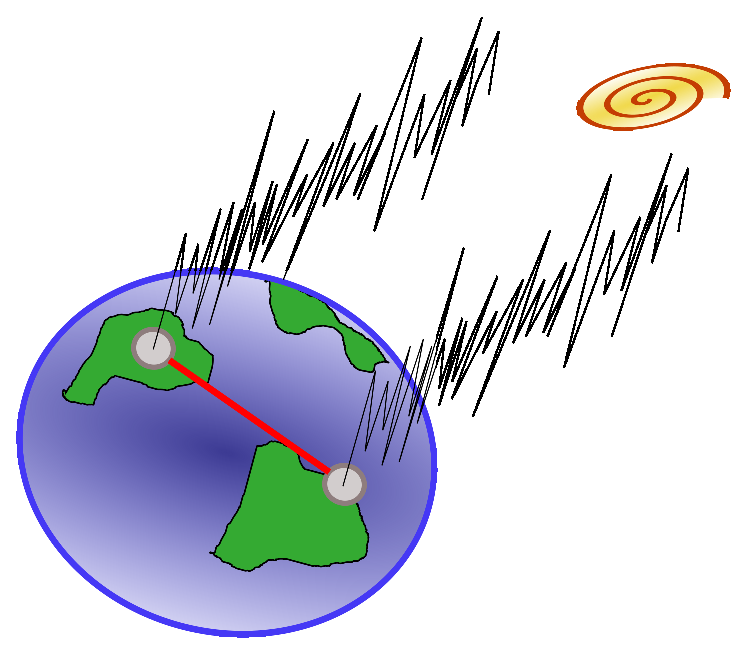
\includegraphics[width=0.8\linewidth]{figure/vlbi_concept}\hspace*{\fill}
\end{centering}
\end{frame}

\begin{frame}{Quasars}
\begin{minipage}[t][][c]{0.48\linewidth}
    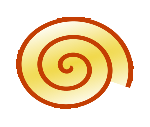
\includegraphics[width=0.7\linewidth]{figure/quasar2} \\
    \vspace*{1em}
    \includegraphics[width=\linewidth]{figure/quasar.jpg}

    \tiny{\hfill\textcopyright~ ESO/M. Kornmesser}
\end{minipage}\hfill
\begin{minipage}[t][][c]{0.5\linewidth}
\begin{itemize}
  \item Active Galactic Nuclei (AGN)
  \item Black hole with an accretion disk
  \item Billions of light years away
  \item About 200 000 known quasars
  \item Approximately 10\% are radio-loud
  \end{itemize}
\end{minipage}
\end{frame}

\begin{frame}{Network stations}
\begin{centering}
    \hfill\includegraphics[width=0.8\linewidth]{figure/ivsnetmap}\hspace*{\fill}
\end{centering}
\end{frame}

\begin{frame}[c]{Purpose}
\huge {Provide \textbf{reference frames} and \textbf{Earth orientation parameters} to enable \textbf{positioning}}
\end{frame}

\begin{frame}{Simple Reference Frame}
    \hfill\includegraphics[width=\linewidth]{figure/tre}\hspace*{\fill}
\end{frame}

\begin{frame}{Terrestrial Reference Frame}
    \hfill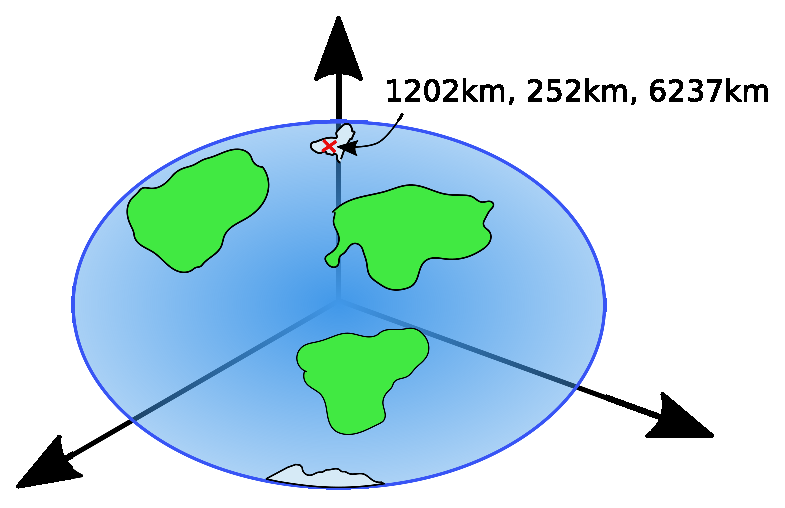
\includegraphics[width=\linewidth]{figure/reference_frame}\hspace*{\fill}
\end{frame}

\begin{frame}{Celestial Reference Frame}
    \hfill\includegraphics[width=0.80\linewidth]{figure/celestial_reference_frame}\hspace*{\fill}
\end{frame}

\begin{frame}{Connecting the reference frames}
\begin{itemize}
\item The quasars are not moving (from our point of view)
\item The celestial reference frame is fixed to the quasars
\item The terrestrial reference frame is fixed to the Earth's crust
\item The Earth orientation parameters connects the two reference frames 
\end{itemize}

\end{frame}

\begin{frame}{Earth Orientation Parameters}
\begin{itemize}
\item Earth's crust is moving (polar motion)
\item Earth spins around its rotation axis (UT1)
\item Earth's rotation axis is wobbling in space (precession/nutation)
\end{itemize}
\end{frame}


\begin{frame}{Organization}
\begin{itemize}
\item Global international collaboration 
\item Governed by International VLBI Service for Geodesy and Astrometry (IVS)
\item Results delivered to International Earth Rotation and Reference
Systems Service (IERS)
\item Historically based on best effort
\item In 2015 the UN General Assembly adopted a resolution for \textbf{A Global Geodetic Reference Frame for
Sustainable Development}
\end{itemize}
\end{frame}

\begin{frame}{Work flow}
\begin{center}
	\includegraphics[height=0.8\textheight]{figure/IVS_flow}
\end{center}
\end{frame}

\begin{frame}{Observing program}
\begin{description}[CONT ]
%\begin{description}[labelindent=1em ,labelwidth=1cm, leftmargin=!, itemindent=0pt, style=sameline]
  \item [\textbf{R}] 24 hour sessions twice a week with 6-12 stations
  \item [\textbf{INT}] Daily 1 hour sessions with 2-3 stations
  \item [\textbf{CONT}] Continuous observations for 2 weeks with largest possible network every three years
  \item [\textbf{T}] One 24 hours sessions 6 times a year with a large global network
  \item [\textbf{Other}] 24 hour sessions with various purposes
\end{description}
\end{frame}

\begin{frame}{Intensive sessions}
\begin{center}
	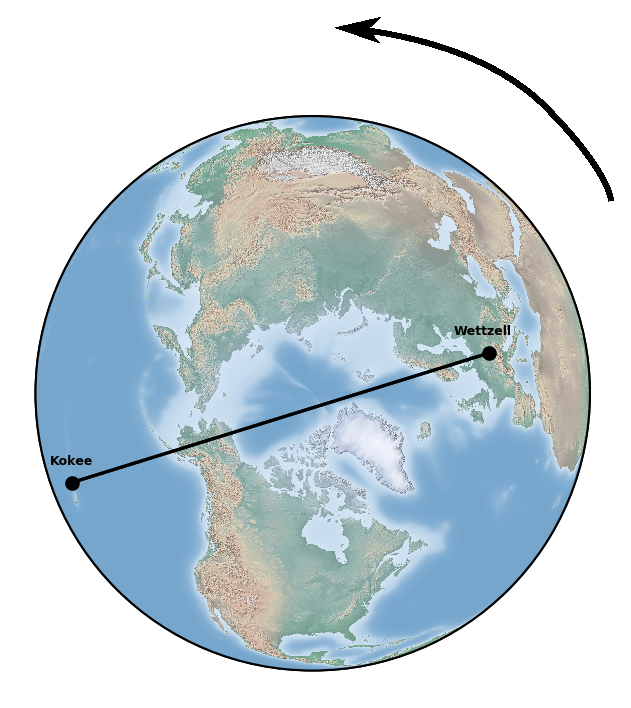
\includegraphics[height=0.8\textheight]{figure/int}
\end{center}
\end{frame}

\begin{frame}{R1-671}
\begin{center}
	\includegraphics[width=0.9\linewidth]{figure/R1671}
\end{center}
\end{frame}

\begin{frame}{2018 Observing program}
\large{Planned and executed so far:}

\vspace*{1em}
\begin{tabularx}{\textwidth}{rXX}
    \textbf{188} & 24hour sessions &  \textbf{50} stations \\
    \textbf{368} & 1hour  sessions &   \textbf{8} stations \\
     \textbf{24} & VGOS   sessions &   \textbf{7} stations \\
\end{tabularx}

\end{frame}

\begin{frame}{VLBI Geodetic Observing System}
The next generation VLBI system

\begin{itemize}
  \item Small and fast antennas for more observations
  \item Broadband receivers for higher sensitivity
  \item Larger network of stations
  \item Operations 24/7
  \item Faster turnaround time 
\end{itemize}
\end{frame}

\begin{frame}{Other techniques}
VLBI alone is not enough to determine a terrestrial reference frame. Data from other measurement techniques are also
needed:
\vspace*{1em}
\begin{itemize}
  \item Satellite Laser Ranging (SLR)
  \item Global Navigation Satellite System (GNSS)
  \item Doppler Orbitography and Radiopositioning Integrated by Satellite (DORIS)
\end{itemize}
\end{frame}

\begin{frame}[fragile,c]{Strengths and weaknesses}
\centering
\footnotesize
\newcolumntype{Y}{>{\centering\arraybackslash}X}
 \begin{tabularx}{\textwidth}{|l|Y|Y|Y|Y|}
	\hline
	\rowcolor{kvlightgreen}	\textbf{Parameter} & \textbf{VLBI} & \textbf{SLR} & \textbf{GNSS} & \textbf{DORIS}\\
  	\hline
    \textbf{Radio sources} & \textbf{X} & & &  \\
	\hline
	\hline
	\textbf{Satellite orbits} &  & \textbf{X} & \textbf{X} & \textbf{X}  \\
    \hline
    \hline
    \textbf{Nutation/Precession} & \textbf{X} & (\textbf{X}) & (\textbf{X}) & \\
    \hline
    \textbf{UT1-UTC} & \textbf{X} & & & \\
    \hline
    \textbf{Length Of Day} & (\textbf{X}) & \textbf{X} & \textbf{X} & \textbf{X} \\
    \hline
    \textbf{Polar motion} & (\textbf{X}) & (\textbf{X}) & \textbf{X} & (\textbf{X}) \\
    \hline
    \hline
    \textbf{Geocenter} & & \textbf{X} & (\textbf{X}) & (\textbf{X}) \\
    \hline
    \textbf{Scale} & \textbf{X} & \textbf{X} & (\textbf{X}) & (\textbf{X}) \\
    \hline
\end{tabularx}
\end{frame}

\part{VLBI with Where}

\begin{frame}{What is \textbf{Where}?}
\begin{itemize}
  \item A new software for geodetic analysis
  \item Where is developed by Kartverket (NMA)
  \item Main focus on VLBI, SLR and GNSS
  \item Based on Python 3 and Cython
  \item Works on multiple platforms
  \item Freely available on GitHub
\end{itemize}
\end{frame}

\begin{frame}{Motivation}
  \begin{itemize}
  \item Use our own data
  \item Evaluate station performance
  \item Build VLBI and SLR expertise and ensure continuity
  \item Contribute to reference frame realization and determination of Earth orientation parameters
  \end{itemize}
\end{frame}

\begin{frame}{VASCC 2015}
 The VLBI Analysis Software Comparison Campaign
\begin{small}
  \begin{itemize}
  \item Compare computed theoretical delay model of different software packages
  \item 11 participants and 6 solutions found to be consistent within 1~mm
  \item We obtained the solution from 2 of the 6 good solutions
  \item When \textbf{Where} matured the VASCC data was analyzed and compared to the good solutions
  \end{itemize}
  \end{small}
\end{frame}

\begin{frame}{\textbf{Where} vs VieVS and c5++}
  \begin{itemize}
    \item 2 networks
    \item 1 minute sampling interval
    \item 16 days
  \end{itemize}
  RMS (in mm) of difference between solutions:
\vspace{1em}
  \begin{tabularx}{\columnwidth}{lrCCC}
  & & \multicolumn{3}{c}{Northern}   \\ \cline{3-5}
  &         & \textbf{Where}  & \textbf{c5++}   & \textbf{VieVS}  \\
  \multirow{3}{*}{\rotatebox[origin=c]{90}{Southern}}
    & \multicolumn{1}{|l}{\textbf{Where}} & $\diamond$ &     $0.49$ &     $0.44$ \\
    & \multicolumn{1}{|l}{\textbf{c5++}}  &     $0.18$ & $\diamond$ &     $0.21$ \\
    & \multicolumn{1}{|l}{\textbf{VieVS}} &     $0.43$ &     $0.39$ & $\diamond$ \\
  \end{tabularx}
\end{frame}

\begin{frame}{IVS analysis center}
\begin{itemize}
  \item Process 24 hours of data regularily within a time limit
  \item Compute station coordinates, radio source coordinates and Earth Orientation Parameters
  \item Submitted 6 solutions to IVS
  \begin{itemize}
   \item Compute solutions based on many years of historical data
   \item Compare with other analysis centers
   \item Fix the problems and repeat
  \end{itemize}
\end{itemize}
\end{frame}

\begin{frame}{Status}
\begin{itemize}
  \item The 6th solution looks good!
  \item Planning a 7th solution to test the transistion to a new file format of the input files
  \item The next step is to start processing of data in near real time 
  \item The operational analysis will be performed at the Control Center in Hønefoss
\end{itemize}
\end{frame}

\begin{frame}{UT1 - UTC}
\begin{centering}
    \includegraphics[width=\linewidth]{figure/iter6_dUT_nma_diff_combi}
\end{centering}
\end{frame}

\part{Basic VLBI Theory}

\begin{frame}{VLBI observation}
\begin{center}
	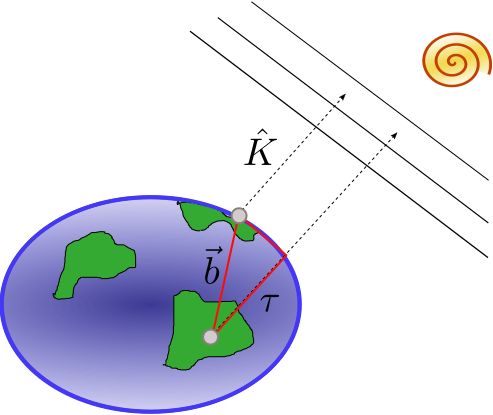
\includegraphics[height=0.8\textheight]{figure/vlbi_concept2}
\end{center}
\end{frame}


\begin{frame}{Time difference $\tau = t_2 - t_1$}
\begin{centering}
    \hfill\includegraphics[width=0.9\linewidth]{figure/corr}\hspace*{\fill}
\end{centering}
\end{frame}

\begin{frame}{VLBI model}
\begin{minipage}[t][][c]{0.40\linewidth}
	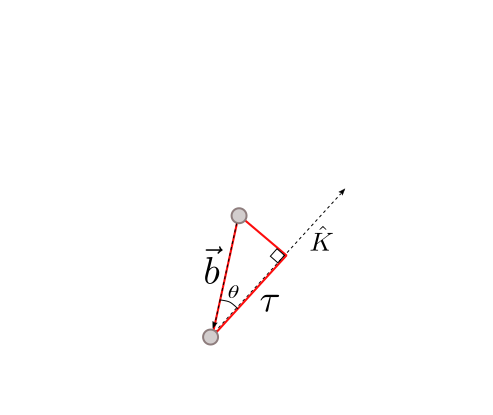
\includegraphics[width=\linewidth]{figure/vlbi_simple}
\end{minipage}
\begin{minipage}[t][][c]{0.5\linewidth}
\vspace{2cm}
\Huge
\begin{equation*}
\tau = - \hat{K} \cdot \vec{b} 
\end{equation*}
\end{minipage}
\end{frame}

\begin{frame}
\begin{block}{Very simple VLBI delay model}
\vspace{-\baselineskip}\setlength\belowdisplayshortskip{0pt}
\begin{equation*}
\tau = - \hat{K} \cdot \vec{b} 
\end{equation*}
\end{block}

But the two vectors, $\vec{b}$ and $\hat{K}$, are defined in different coordinate system. 
\vfill
\pause
\begin{block}{Simple VLBI delay model}
\vspace{-\baselineskip}\setlength\belowdisplayshortskip{0pt}
\begin{equation*}
\tau = - \hat{K} \cdot Q \cdot R \cdot W \cdot \vec{b} 
\end{equation*}
\end{block}
where $QRW$ are three matrices that transform the vector $\vec{b}$ to the same coordinate system as $\hat{K}$.
\end{frame}

\part{Coordinate systems}

\begin{frame}{Barycentric Celestial Reference System}
\begin{minipage}[t][][c]{0.48\linewidth}
	\includegraphics[width=\linewidth]{figure/bcrs}
\end{minipage}
\begin{minipage}[t][][c]{0.5\linewidth}
\begin{itemize}
\item Space fixed
\item Unit sphere
\item Right ascension $\alpha$
\item Declination $\delta$
\item 4D with TCB as time coordinate
\item Orientation aligned to ICRF
%\item Equinox at J2000.0
\end{itemize}
\end{minipage}
\end{frame}


\begin{frame}{Geocentric Terrestrial Reference System}
\begin{minipage}[t][][c]{0.48\linewidth}
	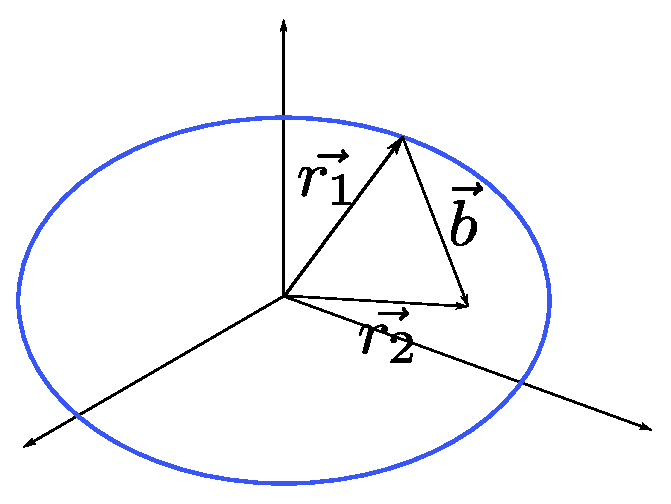
\includegraphics[width=\linewidth]{figure/trs}
\end{minipage}
\begin{minipage}[t][][c]{0.5\linewidth}
\begin{itemize}
\item Earth fixed
\item 4D with TCG as time coordinate 
\item ITRF - 3D - XYZ 
\item SI meter
%\item Orientation given by BIH 1984.0
%\item Orientation's time evolution ensured by NNR to Earth crust
\end{itemize}
\end{minipage}
\end{frame}

\begin{frame}{Geocentric Celestial Reference System}
\begin{minipage}[t][][c]{0.48\linewidth}
	\includegraphics[width=\linewidth]{figure/gcrs}
\end{minipage}
\begin{minipage}[t][][c]{0.5\linewidth}
\begin{itemize}
\item Space Fixed
\item 4D with TCG as time coordinate
\item Orientation aligned to ICRF
%\item General Relativity
\end{itemize}
\end{minipage}
\end{frame}

\begin{frame}{Aberration}
Apparent motion of the quasars due to Earth's velocity
\begin{block}{Aberrated source vector}
\vspace*{-\baselineskip}\setlength\belowdisplayskip{0pt}\setlength\abovedisplayskip{0pt}
\begin{equation*}
\vec{k}_i = \hat{K} + \frac{\vec{V}_{\Earth} + \vec{w}_i}{c} - \hat{K}\frac{\hat{K}\left(\vec{V}_{\Earth} + \vec{w}_i\right)}{c}
\end{equation*}
\end{block}
\begin{description}[$\vec{V}_{\Earth}$]
\item[$\vec{V}_{\Earth}$] - Earth's velocity vector (in the solar system) \\
\item[$\vec{w}_i$] - Station velocity in GCRS \\
\item[$i$] - Station 1 or station 2
\end{description}
\end{frame}

\begin{frame}{Geodetic Latitude, Longitude and Height}
\note{latitude, longitude, height}
\begin{minipage}[t][][c]{0.48\linewidth}
	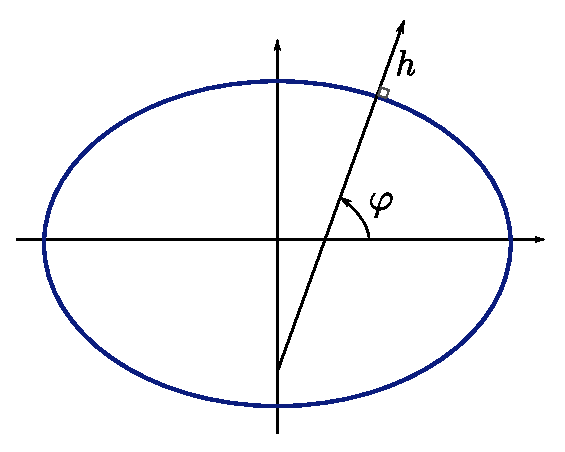
\includegraphics[width=\linewidth]{figure/latitude}
\end{minipage}
\begin{minipage}[t][][c]{0.5\linewidth}
\begin{itemize}
\item GRS80
\item Latitude $\varphi$
\item Longitude $\lambda$
\item Height above ellipsoid $h$
\end{itemize}
\end{minipage}
\end{frame}

\begin{frame}{Topocentric East, North, Up}
Local coordinate system
\begin{block}{ITRS to ENU}
\vspace*{-\baselineskip}\setlength\belowdisplayskip{0pt}\setlength\abovedisplayskip{0pt}
\begin{align*}
\vec{x}_{ENU} &= R_1(\pi/2 - \varphi)R_3(\pi/2 + \lambda) \vec{x}_{ITRS} \\ 
              &= \begin{bmatrix}
                    - \sin\lambda            &   \cos\lambda            & 0 \\
                    - \cos\lambda\sin\varphi & - \sin\lambda\sin\varphi & \cos\varphi \\
                      \cos\lambda\cos\varphi &   \sin\lambda\cos\varphi & \sin\varphi
                 \end{bmatrix}
                 \vec{x}_{ITRS}
\end{align*}
\end{block}
\vfill
East - North plane tangential to ellipsoid at $(\varphi,\lambda)$
\end{frame}


\part{Time}

\begin{frame}{Time scales}
\vfill
\begin{center}
	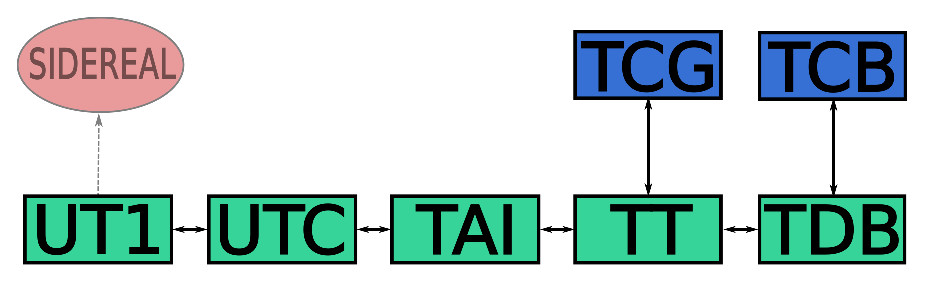
\includegraphics[width=\textwidth]{figure/time}
\end{center}
\end{frame}

\begin{frame}{UT1 - Universal Time}
\begin{center}
	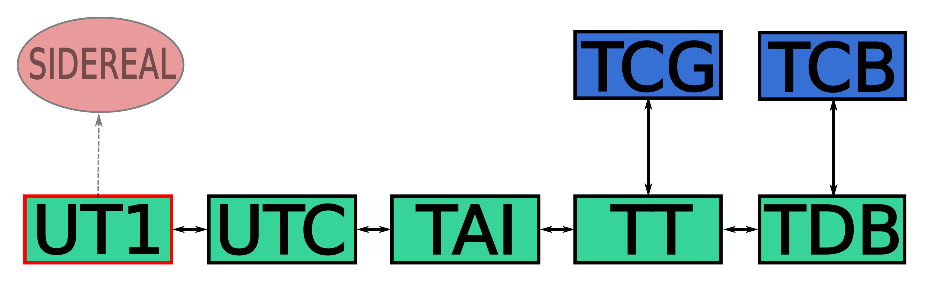
\includegraphics[width=0.8\textwidth]{figure/ut1}
\end{center}
\begin{itemize}
\item Mean Solar Time at $0^{\circ}$ longitude. 
\end{itemize}
\vfill
\begin{block}{Earth Rotation Angle}
\small\vspace*{-\baselineskip}\setlength\belowdisplayskip{0pt}\setlength\abovedisplayskip{0pt}
\begin{align*}
ERA &= 2\Pi(0.7790572732640 + 1.00273781191135448T_u) \\
T_u &= Julian \: \text{UT1} \: date - 2451545.0
\end{align*}
\end{block}
\end{frame}

\begin{frame}{UT1 - UTC}
\begin{center}
	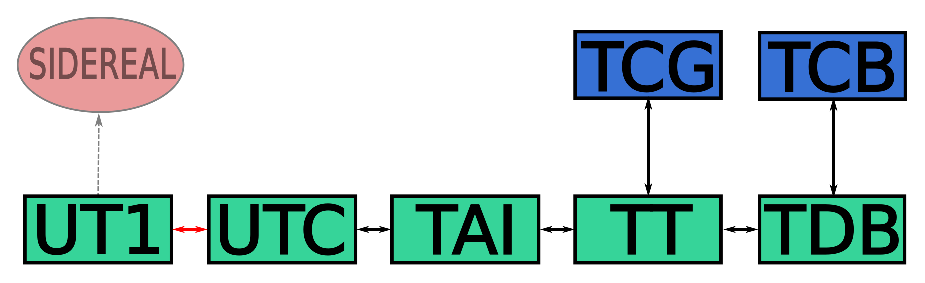
\includegraphics[width=0.8\textwidth]{figure/ut1_utc}
\end{center}
\begin{itemize}
\item Defined to be less than 0.9 seconds 
\end{itemize}
\end{frame}

\begin{frame}{UTC - Coordinated Universal Time}
\begin{center}
	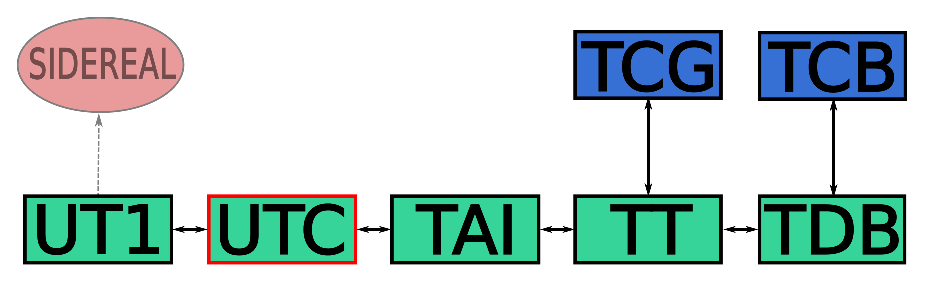
\includegraphics[width=0.8\textwidth]{figure/utc}
\end{center}
\begin{itemize}
\item Atomic time scale based on the SI second.
\item Primary time standard for time keeping in the world
\end{itemize}
\end{frame}

\begin{frame}{UTC - TAI}
\begin{center}
	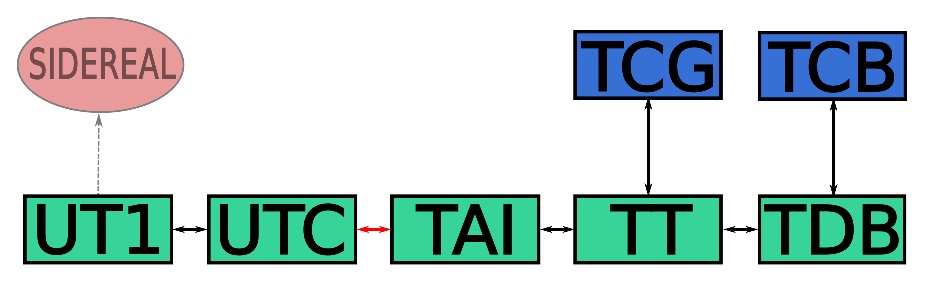
\includegraphics[width=0.8\textwidth]{figure/utc_tai}
\end{center}
\begin{itemize}
\item Leap seconds
\end{itemize}
\end{frame}

\begin{frame}{TAI - International Atomic Time}
\begin{center}
	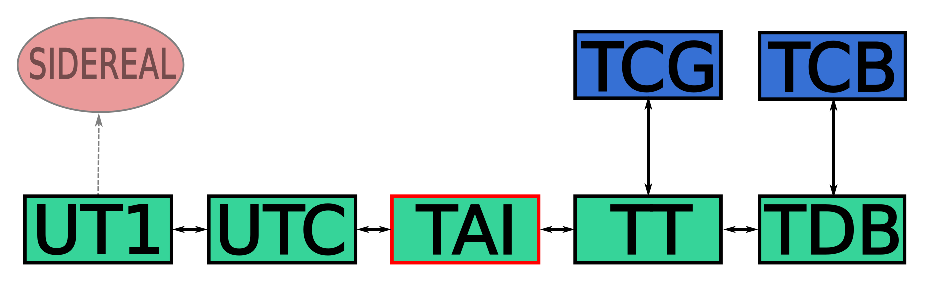
\includegraphics[width=0.8\textwidth]{figure/tai}
\end{center}
\begin{itemize}
\item Atomic time scale based on the SI second.
\item The primary time standard that is realized by a global network of atomic clocks
\item Maintained by BIPM (International Buereau of Weights and Measures)
\end{itemize}
\end{frame}

\begin{frame}{TAI - TT}
\begin{center}
	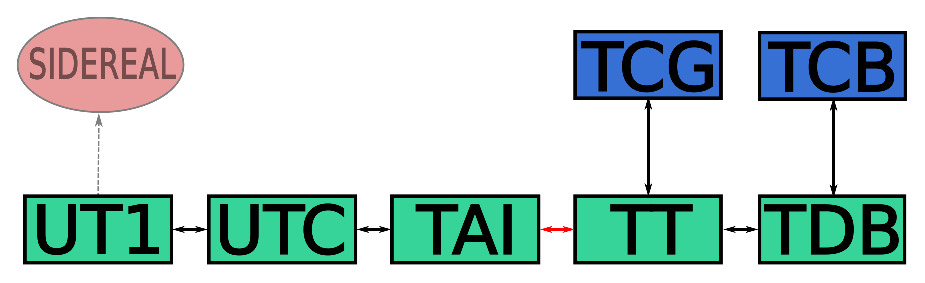
\includegraphics[width=0.8\textwidth]{figure/tai_tt}
\end{center}
\begin{itemize}
\item 32.184 seconds
\item historical reasons for this offset
\end{itemize}
\end{frame}

\begin{frame}{TT - Terrestrial Time}
\begin{center}
	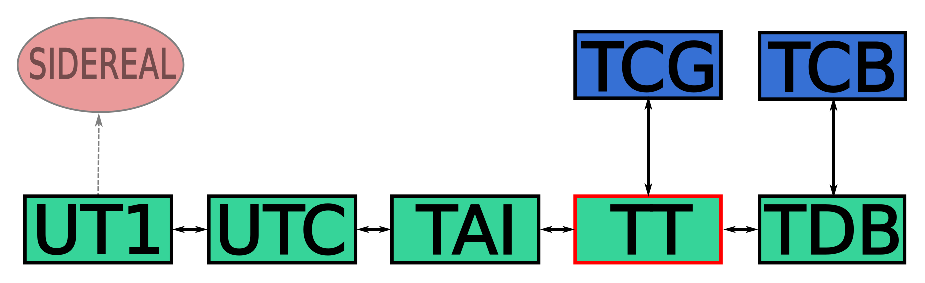
\includegraphics[width=0.8\textwidth]{figure/tt}
\end{center}
\begin{itemize}
\item Approximate time at the geoid using the SI second
\end{itemize}
\end{frame}

\begin{frame}{TT - TCG}
\begin{center}
	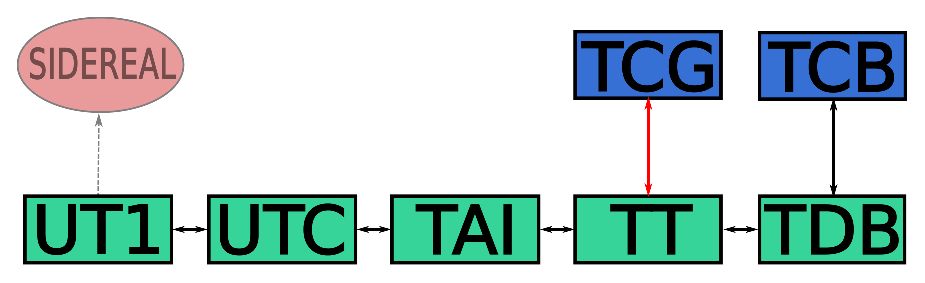
\includegraphics[width=0.8\textwidth]{figure/tt_tcg}
\end{center}
\vspace*{-\baselineskip}
\begin{itemize}
\item Constant rate
\end{itemize}
\begin{block}{TCG - TT}
\small
\vspace*{-\baselineskip}\setlength\belowdisplayskip{0pt}\setlength\abovedisplayskip{0pt}
\begin{align*}
\text{TCG} - \text{TT} &= \left( \frac{L_G}{1 - L_G} \right) \times \left( \text{JD}_\text{TT} - T_0\right) \times 86400 \text{s}\\
T_0 &= 2443144.500372 \\
L_G &= 6.969290134 \times 10^{-10}
\end{align*}
\end{block}
\end{frame}

\begin{frame}{TCG - Geocentric Coordinate Time}
\begin{center}
	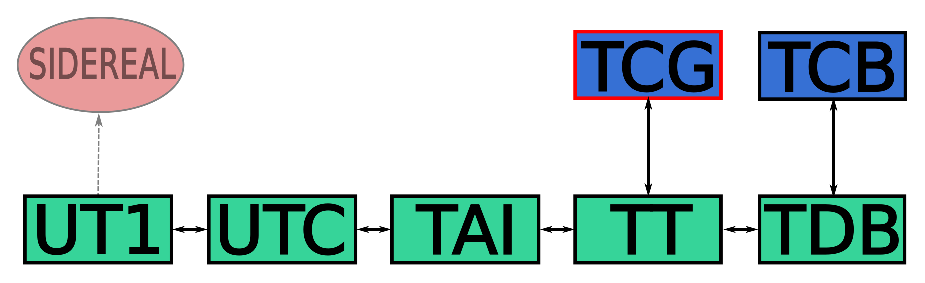
\includegraphics[width=0.8\textwidth]{figure/tcg}
\end{center}
\begin{itemize}
\item Coordinate time
\item No gravitational time dilation from the Earth
\end{itemize}
\end{frame}


\begin{frame}{TT - TDB}
\begin{center}
	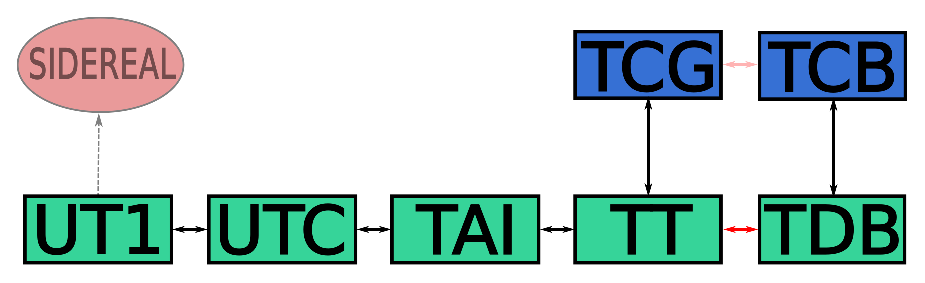
\includegraphics[width=0.8\textwidth]{figure/tt_tdb}
\end{center}
\vspace*{-\baselineskip}
\begin{itemize}
\item 4D transformation
\end{itemize}
\begin{block}{TCB - TCG}
\footnotesize
\vspace*{-\baselineskip}\setlength\belowdisplayskip{0pt}\setlength\abovedisplayskip{0pt}
\begin{align*}
\text{TCB} - \text{TCG} &= \frac{L_C \left(TT - T_0\right) + P(TT) - P(T_0)}{1 - L_B} + 
\frac{\vec{V}_\Earth \left(\vec{X} - \vec{X}_\Earth\right)}{c^2}\\
L_C &= 1.48082686741 \times 10^{-8} \\
P(...) &= \text{Periodic terms}
\end{align*}
\end{block}
\end{frame}

\begin{frame}{TDB - Barycentric Dynamical Time}
\begin{center}
	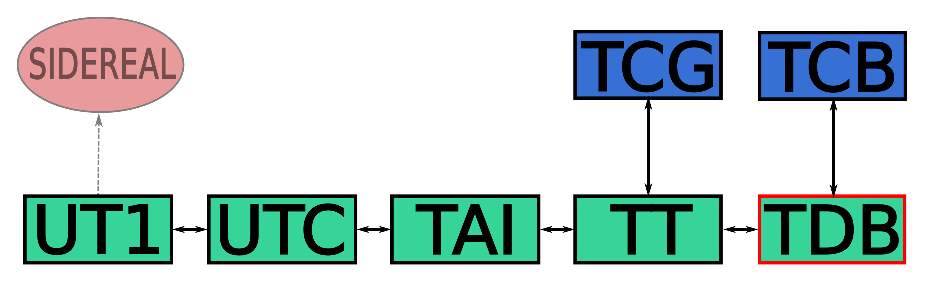
\includegraphics[width=0.8\textwidth]{figure/tdb}
\end{center}
Planet ephemerides
\end{frame}

\begin{frame}{TDB - TCB}
\begin{center}
	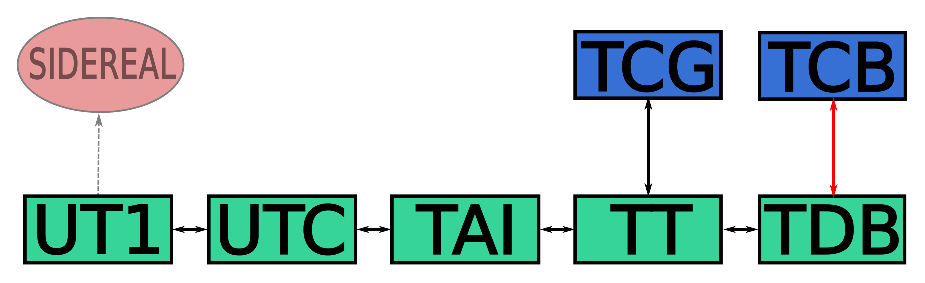
\includegraphics[width=0.8\textwidth]{figure/tdb_tcb}
\end{center}
\vspace*{-\baselineskip}
\begin{itemize}
\item Linear transformation
\end{itemize}
\begin{block}{TDB}
\small
\vspace*{-\baselineskip}\setlength\belowdisplayskip{0pt}\setlength\abovedisplayskip{0pt}
\begin{align*}
\text{TDB} &= \text{TCB} - L_B \times \left( \text{JD}_\text{TCB} - T_0\right) \times 86400 \text{s} + \text{TDB}_0\\
\text{TDB}_0 &= -6.55 \times 10^{-5} \text{s} \\
L_B &= 1.550519768 \times 10^{-8}
\end{align*}
\end{block}
\end{frame}

\begin{frame}{TCB - Barycentric Coordinate Time}
\begin{center}
	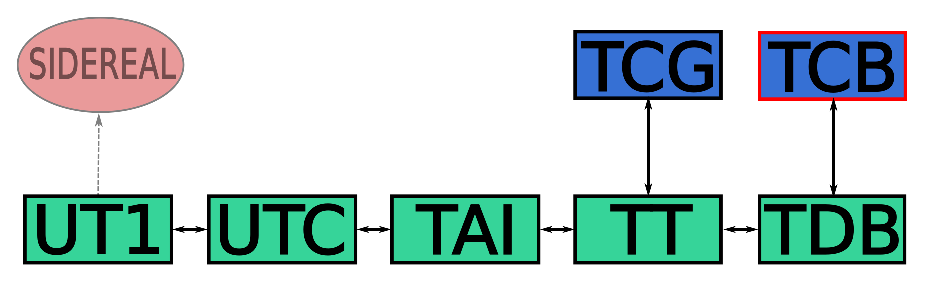
\includegraphics[width=0.8\textwidth]{figure/tcb}
\end{center}
\begin{itemize}
\item Coordinate time
\item No gravitational time dilation from the Solar System
\end{itemize}
\end{frame}

\part{Earth Orientation Parameters}

\begin{frame}{EOP}
\begin{itemize}
\item There are five Earth Orientation Parameters 
\begin{itemize}
\item Two polar motion coordinates
\item One rotation parameter
\item Two precession/nutation coordinates
\end{itemize}
\item The EOP connects the terrestrial reference system to the geocentric celestial reference system
\end{itemize}
\end{frame}

\begin{frame}{Transformation}
\begin{block}{ITRS to GCRS}
\vspace*{-\baselineskip}\setlength\belowdisplayskip{0pt}\setlength\abovedisplayskip{0pt}
\begin{equation*}
\vec{x}_{GCRS}(t) = Q(t) \cdot R(t) \cdot W(t) \cdot \vec{x}_{ITRS}(t) 
\end{equation*}
\end{block}
\vfill
\begin{description}[W ]
\item[$t$] (TT - 2000 Jan 1 12h TT) in days/36525
\item[$Q$] motion of the CIP in the GCRS ($X$, $Y$)
%\begin{itemize}
%\item $x_p$, $x_p$
%\end{itemize}
\item[$R$] rotation of the Earth around the axis of the CIP ($UT1-UTC$)
%\begin{itemize}
%\item UT1
%\end{itemize}
\item[$W$] motion of the CIP in the ITRS ($x_p$, $y_p$)
%\begin{itemize}
%\item $X$, $Y$
%\end{itemize}
\end{description}
\end{frame}


\begin{frame}{Celestial Intermediate Pole}
\begin{quote}
The CIP is an intermediate pole separating, by convention, the motion of the pole of the ITRS in the GCRS into a celestial part and a terrestrial part:
\begin{itemize}
\item the celestial motion of the CIP includes all the terms with periods greater than 2 days in the GCRS
\item the terrestrial motion of the CIP includes all the terms outside the retrograde diurnal band in the ITRS
\end{itemize}
\end{quote}
\end{frame}

\begin{frame}{Nutation/Precession}
\begin{block}{Spherical coordinates}
\vspace*{-\baselineskip}\setlength\belowdisplayskip{0pt}\setlength\abovedisplayskip{0pt}
\begin{align*}
X &= r \sin d \cos E \\
Y &= r \sin d \sin E \\
Z &= r \cos d
\end{align*}
\end{block}
\begin{description}[$d$]
\item[$d$] Polar angle
\item[$E$] Azimuth angle
\item[$r$] Radius (r=1)
\end{description}
\end{frame}

\begin{frame}{Nutation/Precession}
\begin{block}{Motion of CIP in GCRS}
\vspace*{-\baselineskip}\setlength\belowdisplayskip{0pt}\setlength\abovedisplayskip{0pt}
\begin{equation*}
Q(t) = R_3(-E) \cdot R_2(-d) \cdot R_3(E) \cdot R_3(s)
\end{equation*}
\end{block}
\begin{description}[$s$]
\item[$s$] Celestial Intermediate Origin (CIO) locator
\end{description}
\end{frame}

\begin{frame}{Earth rotation}
\begin{block}{Rotation around the CIP}
\vspace*{-\baselineskip}\setlength\belowdisplayskip{0pt}\setlength\abovedisplayskip{0pt}
\begin{equation*}
R(t) = R_3(-ERA)
\end{equation*}
\end{block}
\begin{description}[$ERA$]
\item[$ERA$] Earth Rotation Angle
\end{description}
\end{frame}

\begin{frame}{Polar motion}
\begin{block}{Motion of CIP in ITRS}
\vspace*{-\baselineskip}\setlength\belowdisplayskip{0pt}\setlength\abovedisplayskip{0pt}
\begin{equation*}
W(t) = R_3(-s') \cdot R_2(x_p) \cdot R_1(y_p) 
\end{equation*}
\end{block}
\begin{description}[$s'$]
\item[$s'$] Terrestrial Intermediate Origin (TIO) locator
\end{description}
\end{frame}

\part{VLBI model}

\begin{frame}{VLBI model}

\begin{block}{Simple VLBI delay model}
\vspace{-\baselineskip}\setlength\belowdisplayshortskip{0pt}
\begin{equation*}
\tau_{geometric} = - \hat{K} \cdot Q \cdot R \cdot W \cdot \vec{b} 
\end{equation*}
\end{block}
\vspace*{2em}
All the delay equations are expressed in meters
\end{frame}

\begin{frame}{Conventional VLBI model}
\begin{block}{Actual VLBI delay model}
\vspace*{-\baselineskip}\setlength\belowdisplayskip{0pt}\setlength\abovedisplayskip{0pt}
\begin{align*}
\tau &= \tau _{geometric} + \tau _{grav} + \Delta\tau _{tropo} + \Delta\tau _{axis} \\
     &- \Delta\tau _{thermdef} + \tau _{clock} - \Delta\tau _{cable} + \tau _{iono}
\end{align*}
\end{block}

\begin{block}{Notation}
\vspace*{-\baselineskip}\setlength\belowdisplayshortskip{0pt}
\begin{equation*}
\Delta\tau_{xxx} = \tau_{xxx}(station2) - \tau_{xxx}(station1)
\end{equation*}
\end{block}
\end{frame}


\begin{frame}{Geometric delay}
\begin{block}{Total geometric delay}
\vspace*{-\baselineskip}\setlength\belowdisplayskip{0pt}\setlength\abovedisplayskip{0pt}
\begin{align*}
\tau_{geometric} = \tau_{v} + \tau_{a}
\end{align*}
\end{block}
\begin{description}
\item[$\tau_{v}$] Geometric vacuum delay
\item[$\tau_{a}$] Atmospheric correction term
\end{description}
\end{frame}

\begin{frame}{Geometric delay}
\begin{block}{Vacuum delay}
\small
\vspace*{-\baselineskip}\setlength\belowdisplayskip{0pt}\setlength\abovedisplayskip{0pt}
\begin{align*}
\tau_{v} &= \frac{-\hat{K}\cdot\vec{b}\left[1 - \frac{(1+\gamma)U}{c} -
\frac{\lvert\vec{V}_{\Earth}\rvert^2}{2c^2} - \frac{\vec{V}_{\Earth}\cdot\vec{w}_2}{c^2}\right] - \frac{\vec{V}_{\Earth}\cdot\vec{b}}{c^2}\left(1 + \frac{\hat{K}\cdot\vec{V}_{\Earth}}{2c}\right)} {1 + \frac{\hat{K}\left(\vec{V}_{\Earth} + \vec{w}_2\right) }{c}} \\ %denominator 
\end{align*}
\end{block}
\begin{description}[aa]
\item[$\vec{b}$] baseline vector in GCRS
\item[$\gamma$] post-Newtonian parameter (space curvature)
\item[$U$] gravitational potential from the Sun
\end{description}
\end{frame}

\begin{frame}{Geometric delay}
\begin{block}{Potential from the Sun at the geocenter}
\vspace*{-.5\baselineskip}\setlength\belowdisplayskip{0pt}\setlength\abovedisplayskip{0pt}
\begin{equation*}
U = \frac{GM_{\Sun}}{\lvert\vec{R}_{\Earth_{\Sun}}\rvert}
\end{equation*}
\end{block}
\begin{description}[$\lvert\vec{R}_{\Earth_{\Sun}}\rvert$]
\item[$M_\Sun$] Mass of the Sun
\item[$\lvert\vec{R}_{\Earth_{\Sun}}\rvert$] Distance between the Earth and the Sun
\end{description}
\end{frame}

\begin{frame}{Geometric delay}
\begin{block}{Atmospheric correction term}
\small
\vspace*{-\baselineskip}\setlength\belowdisplayskip{0pt}\setlength\abovedisplayskip{0pt}
\begin{align*}
\tau_{a} &= \delta t_{{atm}_1}\hat{K}\left(\vec{w}_2 -\vec{w}_1\right)
\end{align*}
\end{block}
\begin{description}[$\delta t_{{atm}_1}$]
\item[$\delta t_{{atm}_1}$] troposphere delay at station 1
\end{description}
\end{frame}


\begin{frame}{General relativistic delay}
\begin{block}{Total delay from gravitating bodies}
\vspace*{-\baselineskip}\setlength\belowdisplayskip{0pt}\setlength\abovedisplayskip{0pt}
\begin{align*}
\tau_{grav} &= \frac{\sum_J\tau_{grav_J} + \sum_J\delta\tau_{grav_J}}
{1 + \frac{\hat{K}\left(\vec{V}_{\Earth} + \vec{w}_2\right)}{c}} %denominator 
\end{align*}
\end{block}
\begin{description}[$\delta\tau_{grav_J}$]
\item[$\tau_{grav_J}$] Delay from celestial body $J$
\item[$\delta\tau_{grav_J}$] Higher order delay from celestial body $J$
\end{description}
\end{frame}

\begin{frame}{General relativistic delay}
\begin{block}{Delay from one celestial body}
\vspace*{-\baselineskip}\setlength\belowdisplayskip{0pt}\setlength\abovedisplayskip{0pt}
\begin{align*}
\tau_{grav_J} &= 2\frac{GM_J}{c^2}\ln\frac{\lvert\vec{R}_{1_J}\rvert +
\hat{K}\cdot\vec{R}_{1_J}}{\lvert\vec{R}_{2_J}\rvert + \hat{K}\cdot\vec{R}_{2_J}} \\
\end{align*}
\end{block}
\begin{description}[$\vec{R}_{i_J}$]
\item[$M_J$] Mass of celestial body $J$
\item[$\vec{R}_{i_J}$] Vector from station $i$ to celestial body $J$
\end{description}
\end{frame}


\begin{frame}{General relativistic delay}
\begin{block}{Delay from Earth}
\vspace*{-\baselineskip}\setlength\belowdisplayskip{0pt}\setlength\abovedisplayskip{0pt}
\begin{align*}
\tau_{grav_{\Earth}} &= 2\frac{GM_{\Earth}}{c^2}\ln\frac{\lvert\vec{x}_1\rvert +
\hat{K}\cdot\vec{x}_1}{\lvert\vec{x}_2\rvert + \hat{K}\cdot\vec{x}_2}
\end{align*}
\end{block}
\begin{description}[$M_\Earth$]
\item[$M_\Earth$] Mass of Earth
\item[$\vec{x}_i$] Position vector of station $i$ in GCRS
\end{description}
\end{frame}


\begin{frame}{General relativistic delay}
\begin{block}{Vectors}
\vspace*{-\baselineskip}\setlength\belowdisplayskip{0pt}\setlength\abovedisplayskip{0pt}
\begin{align*}
\vec{X}_i(t_1) &= \vec{X}_{\Earth}(t_1) + \vec{x}_i(t_1) \\
\vec{R}_{1_J} &= \vec{X}_1(t_1) - \vec{X}_J(t_{1_J}) \\
\vec{R}_{2_J} &= \vec{X}_2(t_1) - \frac{\vec{V}_{\Earth}}{c}\left(\hat{K}\cdot\vec{b}\right) - \vec{X}_J(t_{1_J})
\end{align*}
\end{block}
\begin{block}{Time argument}
\vspace*{-\baselineskip}\setlength\belowdisplayskip{0pt}\setlength\abovedisplayskip{0pt}
\begin{align*}
t_{1_J} &= \min\left[t_1,t_1 -\frac{\hat{K}\left(\vec{X}_J(t_1) - \vec{X}_1(t_1)\right)}{c} \right]
\note {min(arrival time at station 1, arrival time at body J)}
\end{align*}
\end{block}
\end{frame}



\begin{frame}{General relativistic delay}
\begin{block}{Higher order relativistic time delay}
\vspace*{-\baselineskip}\setlength\belowdisplayskip{0pt}\setlength\abovedisplayskip{0pt}
\begin{align*}
\delta\tau_{grav_J} &= \frac{4G^2M_J^2}{c^4}\frac{\vec{b}\left(\hat{N}_{1_J} +
\hat{K}\right)}{\left(\lvert\vec{R}_{1_J}\rvert + \vec{R}_{1_J}\cdot\hat{K}\right)^2} \\
\hat{N}_{1_J} &= \frac{\vec{R}_{1_J}}{\lvert\vec{R}_{1_J}\rvert}
\end{align*}
\end{block}
\end{frame}

% \begin{frame}{Aberration}
% \begin{block}{Aberrated source vector}
% \vspace*{-\baselineskip}\setlength\belowdisplayskip{0pt}\setlength\abovedisplayskip{0pt}
% \begin{equation*}
% \vec{k}_i = \hat{K} + \frac{\vec{V}_{\Earth} + \vec{w}_i}{c} - \hat{K}\frac{\hat{K}\left(\vec{V}_{\Earth} + \vec{w}_i\right)}{c}
% \end{equation*}
% \end{block}
% \end{frame}

\begin{frame}{Tropospheric delay}
\begin{block}{Total tropospheric delay at one station}
\vspace*{-\baselineskip}\setlength\belowdisplayskip{0pt}\setlength\abovedisplayskip{0pt}
\begin{align*}
\tau_{tropo} &= m_h(e)\cdot zhd \\
             &+ m_w(e)\cdot zwd \\
             &+ m_g(e)(G_N\cos a + G_E\sin a)
\end{align*}
\end{block}

\begin{block}{Zenith hydrostatic delay}
\vspace*{-\baselineskip}\setlength\belowdisplayskip{0pt}\setlength\abovedisplayskip{0pt}
\begin{align*}
zhd &= \frac{0.0022768P(t)}{1 - 0.00266\cos 2\varphi - 0.00000028h} 
\end{align*}
\end{block}
\end{frame}

\begin{frame}{Tropospheric delay}
\begin{block}{Mapping functions}
\vspace*{-\baselineskip}\setlength\belowdisplayskip{0pt}\setlength\abovedisplayskip{0pt}
\begin{align*}
m_{h,w} &= \frac{1 + \frac{a}{1 + \frac{b}{1 + c}}}{\sin e + \frac{a}{\sin e + {\frac{b}{\sin e + c}}}} \\
m_g &= \frac{1}{\sin e \tan e + 0.0032}
\end{align*}
\end{block}
\end{frame}

\begin{frame}{Delay due to axis offset}

\begin{block}{Different antenna geometry}
\vspace*{-\baselineskip}\setlength\belowdisplayskip{0pt}\setlength\abovedisplayskip{0pt}
\begin{align*}
\tau_{axis_{AZEL}} &= -AO \cos e \\
\tau_{axis_{EQUA}} &= -AO \cos \delta \\
\tau_{axis_{XYNO}} &= -AO \sqrt{1 - (\cos e \cos a)^2} \\
\tau_{axis_{XYEA}} &= -AO \sqrt{1 - (\cos e \sin a)^2}
\end{align*}
\end{block}
\begin{description}[$e, a$]
\item[$e, a$] elevation, azimuth
\item[$\delta$] radio source declination
\item[$AO$] axis offset
\end{description}
\end{frame}

\begin{frame}{Delay due to thermal deformation}

\begin{block}{Different antenna geometry}
\small
\vspace*{-\baselineskip}\setlength\belowdisplayskip{0pt}\setlength\abovedisplayskip{0pt}
\begin{align*}
\tau_{therm} &= \gamma_f (T(t - \Delta t_f) - T_0) h_f \sin e \\
             &+ \gamma_a (T(t - \Delta t_a) - T_0) (h_p \sin e + axis + h_v - F_a h_s)
\end{align*}
\end{block}
\begin{block}{\vspace*{-3ex}}
\vspace*{-\baselineskip}\setlength\belowdisplayskip{0pt}\setlength\abovedisplayskip{0pt}
\begin{align*}
axis_{AZEL} &= AO \sin z \\
axis_{EQUA} &= AO \cos \delta \\
axis_{XYNO} &= AO \sqrt{1 - (\cos e \cos a)^2} \\
axis_{XYEA} &= AO \sqrt{1 - (\cos e \sin a)^2}
%\tau_{therm_{AZEL}} &{\scriptstyle = \gamma_f (T(t - \Delta t_f) - T_0) h_f \sin e} \\
%                    &{\scriptstyle + \gamma_a (T(t - \Delta t_a) - T_0) (h_p \sin e + AO \sin z + h_v - F_a h_s)} \\
%\tau_{therm_{EQUA}} &{\scriptstyle = \gamma_f (T(t - \Delta t_f) - T_0) h_f \sin e} \\
%                    &{\scriptstyle + \gamma_a (T(t - \Delta t_a) - T_0) (h_p \sin e + AO \cos \delta + h_v - F_a h_s)}
%                    % \\
%\tau_{therm_{XYNO}} &{\scriptstyle = \gamma_f (T(t - \Delta t_f) - T_0) h_f \sin e} \\
%                    &{\scriptstyle + \gamma_a (T(t - \Delta t_a) - T_0) (h_p \sin e + AO \sqrt{1 - (\cos e \cos a)^2} +
%                    % h_v - F_a h_s)} \\
%\tau_{therm_{XYEA}} &{\scriptstyle = \gamma_f (T(t - \Delta t_f) - T_0) h_f \sin e} \\
%                    &{\scriptstyle + \gamma_a (T(t - \Delta t_a) - T_0) (h_p \sin e + AO \sqrt{1 - (\cos e \sin a)^2} +
                    % h_v - F_a h_s)}
\end{align*}
\end{block}
\end{frame}


\begin{frame}{Cable delay}
Cable delay, $\tau_{cable}$, is measured at the station and is applied directly to the delay as is.
\end{frame}

\begin{frame}{Ionospheric delay}
In version 4 of the observation files the ionosphere delay on X-band is already computed and can be applied directly as
is.
\vspace*{\baselineskip}
\begin{block}{Ionosphere X-band}
\vspace*{-\baselineskip}\setlength\belowdisplayskip{0pt}\setlength\abovedisplayskip{0pt}
\begin{equation*}
\tau_{iono} = (\tau_X - \tau_S) \frac{f_S^2}{f_X^2 - f_S^2}
\end{equation*}
\end{block}
\begin{description}[$\tau_X, \tau_S$]
\item[$\tau_X, \tau_S$] delay on X-band and S-band
\item[$f_X, f_S$] frequency of X-band and S-band
\end{description}
\end{frame}

\begin{frame}{Delay due to clocks}
One station is selected as reference station and the effect on the delay is then the difference between the reference
clock and clocks at the other stations. The clock model is divided into two parts:
\vspace*{\baselineskip}
\begin{itemize}
  \item One quadratic polynomial for the long trend
  \item One continuous piecewise linear function for the short term variations
\end{itemize}
\end{frame}

\begin{frame}{Delay due to clocks}
\begin{block}{Clock model}
\vspace*{-\baselineskip}\setlength\belowdisplayskip{0pt}\setlength\abovedisplayskip{0pt}
\begin{align*}
\tau_{clock} = \tau_{poly} + \Delta\tau_{clk} \\
\tau_{poly} &= c_0 + c_1\Delta t + c_2\Delta t^2 \\
\Delta\tau_{clk} &= \tau_{clk_2} - \tau_{clk_1}
\end{align*}
\end{block}
\begin{description}[$a_j, b_j$]
\item[$c_i$] polynomial coefficients
\end{description}
\end{frame}

\begin{frame}{Station coordinates}
\begin{block}{Coordinate at observation epoch}
\vspace*{-\baselineskip}\setlength\belowdisplayskip{0pt}\setlength\abovedisplayskip{0pt}
\begin{equation*}
\vec{r}(t) = \vec{r}^{~itrf}(t_0) + \dot{\vec{r}}^{~itrf}(t - t_0) + \delta\vec{r}^{~psd}(t) +
\sum_j\delta\vec{r}^{~j}(t)
\end{equation*}
\end{block}
\begin{description}[$\delta\vec{r}^{~psd}$]
\item[$t_0$] ITRF reference epoch 
\item[$\vec{r}^{~itrf}$] ITRF position
\item[$\dot{\vec{r}}^{~itrf}$] ITRF linear velocity model
\item[$\delta\vec{r}^{~psd}$] ITRF post seismic deformation
\item[$\delta\vec{r}^{~j}$] station displacement model $j$
\end{description}
\end{frame}

\begin{frame}{Station displacements}
\begin{itemize}
  \item Solid Earth tides
  \item Ocean tidal loading
  \item Atmospheric pressure loading
  \item Pole tide
  \item Ocean pole tide
  \item Eccentricity vector
\end{itemize}
\begin{equation*}
\end{equation*}
\end{frame}

\begin{frame}{EOP models}
\begin{itemize}
  \item Zonal tides (already included in IERS UT1)
  \item Diurnal and semi-diurnal variations due to ocean tides
  \item Libration: unmodelled motions with period less than two days 
\end{itemize}
\begin{block}{Corrections}
\small
\vspace*{-\baselineskip}\setlength\belowdisplayskip{0pt}\setlength\abovedisplayskip{0pt}
\begin{align*}
(x_p, y_p) &= (x_p, y_p)_{IERS} + (\Delta x,\Delta y)_{ocean\_tides} + (\Delta x, \Delta y)_{libration}\\
UT1 &= UT1_{IERS} + \Delta UT1_{ocean\_tides} + \Delta UT1_{libration}
\end{align*}
\end{block}
\end{frame}

%\begin{frame}{VASCC}

%\comment{The main goal of the \textbf{V}LBI \textbf{A}nalysis \textbf{S}oftware \textbf{C}omparison \textbf{C}ampaign 2015 is to compare different VLBI analysis software packages on the basis of computed theoretical delay.}

%\begin{equation*}
%\xcancel{observasjon} - modell = residual
%\end{equation*}

%\begin{align*}
%\tau &= \tau _{geometric} + \tau _{grav} + \tau _{tropo} + \tau _{axisoffset} \\
%     &+ \tau _{thermdef} + \xcancel{\tau _{clock}} + \xcancel{\tau _{cable}} + \xcancel{\tau _{iono}}
%\end{align*}
%\end{frame}

\part{Estimation motivation}

\begin{frame}{Parameter estimation}

The VLBI model is some function that depend on a set of parameters $\mathbf{x}$ and the observation epoch $t$
\vspace*{\baselineskip}
\begin{block}{VLBI delay model}
\vspace*{-\baselineskip}\setlength\belowdisplayskip{0pt}\setlength\abovedisplayskip{0pt}
\begin{equation*}
\tau = f(t, \mathbf{x})
\end{equation*}
\end{block}
\end{frame}

\begin{frame}{Stage: Calculate}
%\begin{block}{Goal}
\begin{itemize}
\item Calculate the theoretical delay, $\tau$, based on conventional models and a priori model parameters
$\mathbf{x}_0$.
\item Then compare the calculated value with the observed values, $o$.
\end{itemize}
%\end{block}
\vspace*{\baselineskip}
\begin{block}{Reduced observations}
\vspace*{-\baselineskip}\setlength\belowdisplayskip{0pt}\setlength\abovedisplayskip{0pt}
\begin{equation*}
l(t) = o(t) - f(t, \mathbf{x}_0)
\end{equation*}
\end{block}
\end{frame}

\begin{frame}{Stage: Estimate}
The reduced observations $l(t)$ is different from zero due to:
\begin{itemize}
  \item measurement errors
  \item unmodelled contributions to the delay
  \item wrong a priori model parameters
\end{itemize}
\vspace*{\baselineskip}
The goal of estimation stage is to find corrections $\Delta\mathbf{x}$ to the a priori model parameters $\mathbf{x}_0$
\end{frame}

\begin{frame}{Stage: Estimate}
\begin{block}{Observation equation}
\vspace*{-\baselineskip}\setlength\belowdisplayskip{0pt}\setlength\abovedisplayskip{0pt}
\begin{equation*}
f(t, \mathbf{x}) = o(t) + v(t)
\end{equation*}
\end{block}
\begin{description}[$v(t)$]
\item[$v(t)$] residuals
\end{description}
\vspace*{\baselineskip}
By minimizing the residuals the corrections $\Delta\mathbf{x}$ to the model parameters can be found
\end{frame}

\begin{frame}{Stage: Estimate}
The equation $f(t,\mathbf{x})$ is not necessarily linear, which is required for the estimation
\vspace*{\baselineskip}
\begin{block}{Taylor expansion}
\vspace*{-\baselineskip}\setlength\belowdisplayskip{0pt}\setlength\abovedisplayskip{0pt}
\begin{align*}
f(t,\mathbf{x}) &= f(t,\mathbf{x}_0) + \left.\frac{\partial f(t, \mathbf{x})}{\partial
\mathbf{x}}\right|_{\mathbf{x}=\mathbf{x_0}}\Delta\mathbf{x} \\
                &= f(t,\mathbf{x}_0) + \mathbf{H}\Delta\mathbf{x}
\end{align*}
\end{block}
\begin{description}[$\mathbf{A}$]
\item[$\mathbf{H}$] Partial derivatives of model with respect to model parameters
\end{description}
\end{frame}

\part{Partials}

\begin{frame}{Parameters}

\begin{itemize}
  \item Station positions
  \item Source positions
  \item Earth Orientation Parameters
  \item Clocks
  \item Troposphere
\end{itemize}
\end{frame}

\begin{frame}{Simplifications}
For the computation of partial derivatives the simple VLBI delay model is sufficient
\vspace*{\baselineskip}
\begin{block}{Simple VLBI delay model}
\vspace*{-\baselineskip}\setlength\belowdisplayskip{0pt}\setlength\abovedisplayskip{0pt}
\begin{equation*}
\tau_{geometric} = - \hat{K} \cdot Q \cdot R \cdot W \cdot (\vec{r}_2 - \vec{r}_1)
\end{equation*}
\end{block}
\begin{description}[$\vec{r}_1$]
\item[$\vec{r}_1$] $(x_1, y_1, z_1)^\mathsf{T}$
\item[$\vec{r}_2$] $(x_2, y_2, z_2)^\mathsf{T}$
\item[$\hat{K}$] $(\cos \delta \cos \alpha, \cos \delta \sin \alpha, \sin \delta)^\mathsf{T}$
\end{description}
\end{frame}

\begin{frame}{Station Positions}
\begin{block}{X component}
\vspace*{-\baselineskip}\setlength\belowdisplayskip{0pt}\setlength\abovedisplayskip{0pt}
\begin{align*}
\frac{\partial \tau}{\partial x_1} &= - \hat{K} \cdot Q \cdot R \cdot W \cdot \frac{\partial (\vec{r}_2 -
\vec{r}_1)}{\partial x_1}\\
\frac{\partial \tau}{\partial x_2} &= - \hat{K} \cdot Q \cdot R \cdot W \cdot \frac{\partial (\vec{r}_2 -
\vec{r}_1)}{\partial x_2} 
\end{align*}
\end{block}
\begin{block}{\vspace*{-3ex}}
\vspace*{-\baselineskip}\setlength\belowdisplayskip{0pt}\setlength\abovedisplayskip{5pt}
\begin{align*}
\frac{\partial (\vec{r}_2 -\vec{r}_1)}{\partial x_1} &= (-1, 0, 0)^\mathsf{T} \\
\frac{\partial (\vec{r}_2 -\vec{r}_1)}{\partial x_2} &= (\phantom{-}1, 0, 0)^\mathsf{T}
\end{align*}
\end{block}
\end{frame}

\begin{frame}{Station Positions}
\begin{block}{Y component}
\vspace*{-\baselineskip}\setlength\belowdisplayskip{0pt}\setlength\abovedisplayskip{0pt}
\begin{align*}
\frac{\partial \tau}{\partial x_1} &= - \hat{K} \cdot Q \cdot R \cdot W \cdot \frac{\partial (\vec{r}_2 -
\vec{r}_1)}{\partial y_1}\\
\frac{\partial \tau}{\partial x_2} &= - \hat{K} \cdot Q \cdot R \cdot W \cdot \frac{\partial (\vec{r}_2 -
\vec{r}_1)}{\partial y_2} 
\end{align*}
\end{block}
\begin{block}{\vspace*{-3ex}}
\vspace*{-\baselineskip}\setlength\belowdisplayskip{0pt}\setlength\abovedisplayskip{5pt}
\begin{align*}
\frac{\partial (\vec{r}_2 -\vec{r}_1)}{\partial y_1} &= (0, -1, 0)^\mathsf{T} \\
\frac{\partial (\vec{r}_2 -\vec{r}_1)}{\partial y_2} &= (0, \phantom{-}1, 0)^\mathsf{T}
\end{align*}
\end{block}
\end{frame}

\begin{frame}{Station Positions}
\begin{block}{Z component}
\vspace*{-\baselineskip}\setlength\belowdisplayskip{0pt}\setlength\abovedisplayskip{0pt}
\begin{align*}
\frac{\partial \tau}{\partial z_1} &= - \hat{K} \cdot Q \cdot R \cdot W \cdot \frac{\partial (\vec{r}_2 -
\vec{r}_1)}{\partial z_1}\\
\frac{\partial \tau}{\partial z_2} &= - \hat{K} \cdot Q \cdot R \cdot W \cdot \frac{\partial (\vec{r}_2 -
\vec{r}_1)}{\partial z_2} 
\end{align*}
\end{block}
\begin{block}{\vspace*{-3ex}}
\vspace*{-\baselineskip}\setlength\belowdisplayskip{0pt}\setlength\abovedisplayskip{5pt}
\begin{align*}
\frac{\partial (\vec{r}_2 -\vec{r}_1)}{\partial z_1} &= (0, 0, -1)^\mathsf{T} \\
\frac{\partial (\vec{r}_2 -\vec{r}_1)}{\partial z_2} &= (0, 0, \phantom{-}1)^\mathsf{T}
\end{align*}
\end{block}
\end{frame}

\begin{frame}{Source Positions}
\begin{block}{Right ascension and declination}
\vspace*{-\baselineskip}\setlength\belowdisplayskip{0pt}\setlength\abovedisplayskip{0pt}
\begin{align*}
\frac{\partial \tau}{\partial \alpha} &= - \frac{\partial \hat{K}}{\partial \alpha} \cdot Q \cdot R \cdot W \cdot
\vec{b} \\
\frac{\partial \tau}{\partial \delta} &= - \frac{\partial \hat{K}}{\partial \delta} \cdot Q \cdot R \cdot W \cdot
\vec{b}
\end{align*}
\end{block}
\begin{block}{\vspace*{-3ex}}
\vspace*{-\baselineskip}\setlength\belowdisplayskip{0pt}\setlength\abovedisplayskip{5pt}
\begin{align*}
%-cos_dec * sin_ra, cos_dec * cos_ra, zero
\frac{\partial \hat{K}}{\partial \alpha} &= (-\cos \delta \sin \alpha, \cos \delta \cos \alpha, 0)^\mathsf{T} \\
%-sin_dec * cos_ra, -sin_dec * sin_ra, cos_dec
\frac{\partial \hat{K}}{\partial \delta} &= (-\sin \delta \cos \alpha, -\sin \delta \sin \alpha, \cos \delta)^\mathsf{T}
\end{align*}
\end{block}
\end{frame}

\begin{frame}{UT1-UTC}
\begin{block}{dUT1}
\vspace*{-\baselineskip}\setlength\belowdisplayskip{0pt}\setlength\abovedisplayskip{0pt}
\begin{align*}
\frac{\partial \tau}{\partial dUT1} &= - \hat{K} \cdot Q \frac{\partial R}{\partial dUT1} \cdot W
\cdot \vec{b}
\end{align*}
\end{block}
\begin{block}{\vspace*{-3ex}}
\vspace*{-\baselineskip}\setlength\belowdisplayskip{0pt}\setlength\abovedisplayskip{5pt}
\begin{align*}
%-rotation.dR3(-ERA(time)) * constant.omega
\frac{\partial R}{\partial dUT1} &= \frac{\partial R_3(-ERA)}{\partial dUT1}
= \frac{\partial R_3(-ERA)}{\partial ERA}\cdot \frac{\partial -ERA}{\partial dUT1} \\
&= -\frac{\partial R_3(-ERA)}{\partial ERA}\cdot \omega
\end{align*}
\end{block}
\begin{description}[$\omega$]
\item[$\omega$] Nominal mean Earth's angular velocity
\end{description}
\end{frame}

\begin{frame}{Length Of Day}
\begin{block}{LOD}
\vspace*{-\baselineskip}\setlength\belowdisplayskip{0pt}\setlength\abovedisplayskip{0pt}
\begin{align*}
\frac{LOD}{1 day} &= - \frac{\mathrm{d}}{\mathrm{d}t} (UT1 - UTC) = - \dot{dUT1}
\end{align*}
\end{block}
\begin{block}{Offset and rate}
\vspace*{-\baselineskip}\setlength\belowdisplayskip{0pt}\setlength\abovedisplayskip{5pt}
\begin{align*}
%-rotation.dR3(-ERA(time)) * constant.omega
UT1 = {dUT1_0} + \dot{dUT1}\Delta t
\end{align*}
\end{block}
\end{frame}

\begin{frame}{Length Of Day}
\begin{block}{LOD}
\vspace*{-\baselineskip}\setlength\belowdisplayskip{0pt}\setlength\abovedisplayskip{0pt}
\begin{align*}
\frac{\partial \tau}{\partial LOD} &= - \hat{K} \cdot Q \frac{\partial R}{\partial LOD} \cdot W
\cdot \vec{b}
\end{align*}
\end{block}
\begin{block}{\vspace*{-3ex}}
\vspace*{-\baselineskip}\setlength\belowdisplayskip{0pt}\setlength\abovedisplayskip{5pt}
\begin{align*}
%rotation.dR3(-ERA(time)) * constant.omega
\frac{\partial R}{\partial LOD} &= \frac{\partial R_3(-ERA)}{\partial LOD}
= \frac{\partial R_3(-ERA)}{\partial ERA}\cdot \frac{\partial -ERA}{\partial LOD} \\
&= -\frac{\partial R_3(-ERA)}{\partial ERA}\cdot \frac{\partial -ERA}{\partial dUT1} \cdot \frac{\partial dUT1}{\partial
LOD} \\
&= -\frac{\partial R_3(-ERA)}{\partial ERA}\cdot \omega \cdot -1
= \frac{\partial R_3(-ERA)}{\partial ERA}\cdot \omega
\end{align*}
\end{block}
\end{frame}

\begin{frame}{Polar motion}
\begin{block}{X-pole}
\vspace*{-\baselineskip}\setlength\belowdisplayskip{0pt}\setlength\abovedisplayskip{0pt}
\begin{align*}
%-(src_dir @ sofa.Q(dset.time) @ sofa.R(dset.time) @ sofa.dW_dxp(dset.time) @ baseline)[:, 0, 0]
\frac{\partial \tau}{\partial x_p} &= - \hat{K} \cdot Q \cdot R \cdot \frac{\partial W}{\partial x_p}
\cdot \vec{b}
\end{align*}
\end{block}
\begin{block}{\vspace*{-3ex}}
\vspace*{-\baselineskip}\setlength\belowdisplayskip{0pt}\setlength\abovedisplayskip{5pt}
\begin{align*}
\frac{\partial W}{\partial x_p} &= \frac{\partial }{\partial x_p} (R_3(s') \cdot R_2(x_p) \cdot R_1(y_p)) \\
&= R_3(s') \cdot \frac{\partial R_2(x_p)}{\partial x_p} \cdot R_1(y_p) 
%rotation.R3(-s_prime(time)) @ rotation.R2(xp(time)) @ rotation.R1(yp(time))
\end{align*}
\end{block}
\end{frame}

\begin{frame}{Polar motion}
\begin{block}{Y-pole}
\vspace*{-\baselineskip}\setlength\belowdisplayskip{0pt}\setlength\abovedisplayskip{0pt}
\begin{align*}
%-(src_dir @ sofa.Q(dset.time) @ sofa.R(dset.time) @ sofa.dW_dyp(dset.time) @ baseline)[:, 0, 0]
\frac{\partial \tau}{\partial y_p} &= - \hat{K} \cdot Q \cdot R \cdot \frac{\partial W}{\partial y_p}
\cdot \vec{b}
\end{align*}
\end{block}
\begin{block}{\vspace*{-3ex}}
\vspace*{-\baselineskip}\setlength\belowdisplayskip{0pt}\setlength\abovedisplayskip{5pt}
\begin{align*}
%rotation.R3(-s_prime(time)) @ rotation.R2(xp(time)) @ rotation.dR1(yp(time))
\frac{\partial W}{\partial y_p} &= \frac{\partial }{\partial y_p} (R_3(s') \cdot R_2(x_p) \cdot R_1(y_p)) \\
&= R_3(s') \cdot R_2(x_p) \cdot  \frac{\partial R_1(y_p)}{\partial y_p} 
\end{align*}
\end{block}
\end{frame}

\begin{frame}{Polar motion rate}
\begin{block}{Offset and rate}
\vspace*{-\baselineskip}\setlength\belowdisplayskip{0pt}\setlength\abovedisplayskip{5pt}
\begin{align*}
x_p = x_{p_0} + \dot{x_p}\Delta t \\
x_p = x_{y_0} + \dot{x_y}\Delta t
\end{align*}
\end{block}
\begin{block}{\vspace*{-3ex}}
\vspace*{-\baselineskip}\setlength\belowdisplayskip{0pt}\setlength\abovedisplayskip{0pt}
\begin{align*}
\frac{\partial \tau}{\partial \dot{x_p}} &= - \hat{K} \cdot Q \cdot R \cdot \frac{\partial W}{\partial x_p} \Delta t
\cdot \vec{b}\\
\frac{\partial \tau}{\partial \dot{y_p}} &= - \hat{K} \cdot Q \cdot R \cdot \frac{\partial W}{\partial y_p} \Delta t \cdot \vec{b}
\end{align*}
\end{block}
\end{frame}

\begin{frame}{Nutation/Precession}
\begin{block}{X and Y}
\vspace*{-\baselineskip}\setlength\belowdisplayskip{0pt}\setlength\abovedisplayskip{0pt}
\begin{align*}
%-(src_dir @ sofa.Q(dset.time) @ sofa.R(dset.time) @ sofa.dW_dyp(dset.time) @ baseline)[:, 0, 0]
\frac{\partial \tau}{\partial X} &= - \hat{K} \cdot \frac{\partial Q}{\partial X} \cdot R \cdot W \cdot \vec{b} \\
\frac{\partial \tau}{\partial Y} &= - \hat{K} \cdot \frac{\partial Q}{\partial Y} \cdot R \cdot W \cdot \vec{b}
\end{align*}
\end{block}
\begin{block}{\vspace*{-3ex}}
\vspace*{-\baselineskip}\setlength\belowdisplayskip{0pt}\setlength\abovedisplayskip{0pt}
\begin{align*}
\frac{\partial Q}{\partial X} &= \frac{\partial }{\partial X} (R_3(-E) \cdot R_2(-d) \cdot R_3(E) \cdot R_3(s)) \\
\frac{\partial Q}{\partial Y} &= \frac{\partial }{\partial Y} (R_3(-E) \cdot R_2(-d) \cdot R_3(E) \cdot R_3(s)) 
\end{align*}
\end{block}
\end{frame}

\begin{frame}{Nutation/Precession}
\begin{block}{X-component}
\vspace*{-\baselineskip}\setlength\belowdisplayskip{0pt}\setlength\abovedisplayskip{0pt}
\begin{align*}
%          dR3_mE @  R2_md @  R3_E @  R3_s * (-dE_dX(time))
%        +  R3_mE @ dR2_md @  R3_E @  R3_s * (-dd_dX(time))
%        +  R3_mE @  R2_md @ dR3_E @  R3_s * ( dE_dX(time))
%        +  R3_mE @  R2_md @  R3_E @ dR3_s * ( ds_dX(time))
\frac{\partial Q}{\partial X}
&= \frac{\partial R_3(-E)}{\partial E} \cdot (-\frac{\partial E}{\partial X}) \cdot R_2(-d) \cdot R_3(E) \cdot R_3(s) \\
&+ R_3(-E) \cdot \frac{\partial R_2(-d)}{\partial X} \cdot (-\frac{\partial d}{\partial X})\cdot R_3(E) \cdot R_3(s) \\
&+ R_3(-E) \cdot R_2(-d) \cdot \frac{\partial R_3(E)}{\partial E} \cdot \frac{\partial E}{\partial X} \cdot R_3(s)\\
&+ R_3(-E) \cdot R_2(-d) \cdot R_3(E) \cdot \frac{\partial R_3(s)}{\partial s} \cdot \frac{\partial s}{\partial X}
\end{align*}
\end{block}
\end{frame}

\begin{frame}{Nutation/Precession}
\begin{block}{Y-component}
\vspace*{-\baselineskip}\setlength\belowdisplayskip{0pt}\setlength\abovedisplayskip{0pt}
\begin{align*}
%          dR3_mE @  R2_md @  R3_E @  R3_s * (-dE_dX(time))
%        +  R3_mE @ dR2_md @  R3_E @  R3_s * (-dd_dX(time))
%        +  R3_mE @  R2_md @ dR3_E @  R3_s * ( dE_dX(time))
%        +  R3_mE @  R2_md @  R3_E @ dR3_s * ( ds_dX(time))
\frac{\partial Q}{\partial Y}
&= \frac{\partial R_3(-E)}{\partial E} \cdot (-\frac{\partial E}{\partial Y}) \cdot R_2(-d) \cdot R_3(E) \cdot R_3(s) \\
&+ R_3(-E) \cdot \frac{\partial R_2(-d)}{\partial Y} \cdot (-\frac{\partial d}{\partial Y})\cdot R_3(E) \cdot R_3(s) \\
&+ R_3(-E) \cdot R_2(-d) \cdot \frac{\partial R_3(E)}{\partial E} \cdot \frac{\partial E}{\partial Y} \cdot R_3(s)\\
&+ R_3(-E) \cdot R_2(-d) \cdot R_3(E) \cdot \frac{\partial R_3(s)}{\partial s} \cdot \frac{\partial s}{\partial Y}
\end{align*}
\end{block}
\end{frame}

\begin{frame}{Nutation/Precession}
\begin{block}{Intermediate partials}
\vspace*{-\baselineskip}\setlength\belowdisplayskip{0pt}\setlength\abovedisplayskip{0pt}
\begin{align*}
%(-Y(time) / (X(time) ** 2 + Y(time) ** 2))[:, None, None] (X(time) / (X(time) ** 2 + Y(time) ** 2))[:, None, None]
\frac{\partial E}{\partial X} &= \frac{-Y}{X^2 + Y^2} \qquad & \frac{\partial E}{\partial Y} &= \frac{X}{X^2 + Y^2} \\
%(X(time) / (Z(time) * np.sqrt(X(time) ** 2 + Y(time) ** 2)))[:, None, None]
%(Y(time) / (Z(time) * np.sqrt(X(time) ** 2 + Y(time) ** 2)))[:, None, None]
\frac{\partial d}{\partial X} &= \frac{X}{Z\sqrt{X^2 + Y^2}} \qquad &\frac{\partial d}{\partial Y} &=
\frac{Y}{Z\sqrt{X^2 + Y^2}}\\
%(-Y(time) / 2)[:, None, None]
%(-X(time) / 2)[:, None, None]
\frac{\partial s}{\partial X} &= \frac{-Y}{2} \qquad & \frac{\partial s}{\partial Y} &= \frac{-X}{2}
\end{align*}
\end{block}
\end{frame}

\begin{frame}{Clocks}
\begin{block}{CPWL clock model}
\vspace*{-\baselineskip}\setlength\belowdisplayskip{0pt}\setlength\abovedisplayskip{0pt}
\begin{align*}
\Delta\tau_{clk} &= \tau_{{clk}_2} - \tau_{{clk}_1}
\end{align*}
\end{block}
\begin{block}{\vspace*{-3ex}}
\vspace*{-\baselineskip}\setlength\belowdisplayskip{0pt}\setlength\abovedisplayskip{0pt}
\begin{align*}
\frac{\partial \Delta\tau_{clk}}{\partial \tau_{{clk}_1}} &= -1 \\
\frac{\partial \Delta\tau_{clk}}{\partial \tau_{{clk}_2}} &= \phantom{-}1 
\end{align*}
\end{block}
\end{frame}

\begin{frame}{Troposphere}
\begin{block}{Zenith wet delay}
\vspace*{-\baselineskip}\setlength\belowdisplayskip{0pt}\setlength\abovedisplayskip{0pt}
\begin{align*}
\Delta\tau_{zwd} &= \tau_{{zwd}_2} - \tau_{{zwd}_1}\\
 &= m_{w_2}(e) \cdot zwd_2 - m_{w_1}(e) \cdot zwd_1
\end{align*}
\end{block}
\begin{block}{\vspace*{-3ex}}
\vspace*{-\baselineskip}\setlength\belowdisplayskip{0pt}\setlength\abovedisplayskip{0pt}
\begin{align*}
\frac{\partial \Delta\tau_{zwd}}{\partial {zwd}_1} &= -m_{w_1}(e)\\ 
\frac{\partial \Delta\tau_{zwd}}{\partial {zwd}_2} &= \phantom{-}m_{w_2}(e) 
\end{align*}
\end{block}
\end{frame}

\begin{frame}{Troposphere}
\begin{block}{North gradient}
\vspace*{-\baselineskip}\setlength\belowdisplayskip{0pt}\setlength\abovedisplayskip{0pt}
\begin{align*}
%m_g(e)(G_N\cos a + G_E\sin a)
\Delta\tau_{G_N} &= \tau_{{G_N}_2} - \tau_{{G_N}_1}\\
 &= m_{g_2}(e) \cdot G_{N_2}\cos a - m_{g_1}(e) \cdot G_{N_1}\cos a
\end{align*}
\end{block}
\begin{block}{\vspace*{-3ex}}
\vspace*{-\baselineskip}\setlength\belowdisplayskip{0pt}\setlength\abovedisplayskip{0pt}
\begin{align*}
\frac{\partial \Delta\tau_{G_N}}{\partial {G_N}_1} &= -m_{g_1}(e)\cdot \cos a\\ 
\frac{\partial \Delta\tau_{G_N}}{\partial {G_N}_2} &= \phantom{-}m_{g_2}(e) \cdot \cos a 
\end{align*}
\end{block}
\end{frame}

\begin{frame}{Troposphere}
\begin{block}{East gradient}
\vspace*{-\baselineskip}\setlength\belowdisplayskip{0pt}\setlength\abovedisplayskip{0pt}
\begin{align*}
%m_g(e)(G_N\cos a + G_E\sin a)
\Delta\tau_{G_E} &= \tau_{{G_E}_2} - \tau_{{G_E}_1}\\
 &= m_{g_2}(e) \cdot G_{E_2}\sin a - m_{g_1}(e) \cdot G_{E_1}\sin a
\end{align*}
\end{block}
\begin{block}{\vspace*{-3ex}}
\vspace*{-\baselineskip}\setlength\belowdisplayskip{0pt}\setlength\abovedisplayskip{0pt}
\begin{align*}
\frac{\partial \Delta\tau_{G_E}}{\partial {G_E}_1} &= -m_{g_1}(e)\cdot \sin a\\ 
\frac{\partial \Delta\tau_{G_E}}{\partial {G_E}_2} &= \phantom{-}m_{g_2}(e) \cdot \sin a 
\end{align*}
\end{block}
\end{frame}

\part{Estimation algorithm}

\begin{frame}{Estimation}
Common methods:
\begin{itemize}
\item Least squares 
\item Kalman filter
\end{itemize}
\vspace*{\baselineskip}
This presentation:
\begin{itemize}
  \item Kalman filter with a Modified Bryson-Frazier smoother
\end{itemize} 
\end{frame}

\begin{frame}{Parameters}
The parameters are divided into two groups:
\begin{itemize}
  \item Constant parameters
  \item Continuous piecewise linear parameters
\end{itemize}
\end{frame}

\begin{frame}{Constant parameters}
\begin{itemize}
  \item One value is estimated for the entire session
  \item This value is representative for the epoch at the middle of the session
\end{itemize}
\end{frame}

\begin{frame}{Continuous piecewise linear parameters}
\begin{itemize}
  \item Estimated as $n$ linear segments
  \item The segments are forced to be connected to each other
  \item The time span of each segment may vary for each parameter
  \item One segment is described by an offset $b$ and a rate $a$
\end{itemize}
\end{frame}

\begin{frame}{State vector}
\begin{align*}
\mathbf{x} =
	\begin{bmatrix}
	\mathbf{x}_{const}     \\
	\mathbf{x}_{cpwl~}     \\
	\end{bmatrix}
\end{align*}
\begin{minipage}[c][][c]{0.48\linewidth}
\begin{align*}
\mathbf{x}_{const} =
	\begin{bmatrix}
	{{sta1_x}}     \\
	\ldots \\
	{{src5_\alpha}}     \\
	\ldots \\
	{UT1~}
	\end{bmatrix}
\end{align*}
\end{minipage}
\begin{minipage}[c][][c]{0.48\linewidth}
\begin{align*}
\mathbf{x}_{cpwl} =
	\begin{bmatrix}
	{{clk1_b}} \\
	{{clk1_a}} \\
	\ldots \\
	{{zwd5_b}} \\
	{{zwd5_a}} \\
	\ldots \\
	\end{bmatrix}
\end{align*}
\end{minipage}
\end{frame}

\begin{frame}{Kalman filter}
\begin{itemize}
  \item Sequential estimator
  \item $j=0$ represent a priori values
  \item $j>0$ represent observation number $j$
  \item $\tilde{\mathbf{x}}$ represents predicted values
  \item $\hat{\mathbf{x}}$ represents estimated values 
  \item $\mathbf{x}*$ represents smoothed values
\end{itemize}
\end{frame}

\begin{frame}{Kalman filter time update}
\begin{align*}
\tilde{\mathbf{x}}_{j+1} &= \mathbf{\Phi}_j \hat{\mathbf{x}}_j\\
\tilde{\mathbf{P}}_{j+1} &= \mathbf{\Phi}_j \hat{\mathbf{P}}_j \mathbf{\Phi}_j^\mathsf{T} + \mathbf{Q}_j
\end{align*}
\vspace*{\baselineskip}
\begin{description}[$\mathbf{\Phi}$]
\item[$\mathbf{\Phi}$] State transition matrix
\item[$\mathbf{P}$] Covariance matrix
\item[$\mathbf{Q}$] Process noise covariance
\end{description}
\end{frame}

\begin{frame}{State transition matrix}
\begin{align*}
\mathbf{\Phi}_j =
\left[\begin{array}{ccc:ccccc}
1      & \ldots & 0      & 0      & \ldots     & \ldots & \ldots & 0          \\
\vdots & \ddots & \vdots & 0      & \ldots     & \ldots & \ldots & 0          \\
0      & \ldots & 1      & 0      & \ldots     & \ldots & \ldots & 0          \\ \hdashline
0      & 0      & 0      & 1      & \Delta t_j & \ldots & \ldots & 0          \\
\vdots & \vdots & \vdots & 0      & 1          & 0      & \ddots & 0          \\
\vdots & \vdots & \vdots & \vdots & \ddots     & \ddots & \vdots & 0          \\
\vdots & \vdots & \vdots & \vdots & \ddots     & \ddots & 1      & \Delta t_j \\
0      & 0      & 0      & 0      & \ldots     & \ldots & 0      & 1
\end{array}\right]
\end{align*}
\end{frame}

\begin{frame}{Process noise covariance}
\begin{align*}
\mathbf{Q}_j =
\left[\begin{array}{ccc:ccccc}
0      & \ldots & 0      & 0      & \ldots     & \ldots & \ldots & 0 \\
\vdots & \ddots & \vdots & 0      & \ldots     & \ldots & \ldots & 0 \\
0      & \ldots & 0      & 0      & \ldots     & \ldots & \ldots & 0 \\ \hdashline
0      & 0      & 0      & 0      & 0          & \ldots & \ldots & 0 \\
\vdots & \vdots & \vdots & 0      & q_i & \ddots & \ddots & 0 \\
\vdots & \vdots & \vdots & \vdots & \ddots     & \ddots & \vdots & 0 \\
\vdots & \vdots & \vdots & \vdots & \ddots     & \ddots & 0      & 0 \\
0      & 0      & 0      & 0      & \ldots     & \ldots & 0      & q_u
\end{array}\right]
\end{align*}
\end{frame}

\begin{frame}{Kalman filter measurement update}
\vspace*{-2.5\baselineskip}
\begin{align*}
\hat{\mathbf{x}}_j &= \tilde{\mathbf{x}}_j + \mathbf{K}_j\mathbf{z}_j\\
\hat{\mathbf{P}}_j &= (\mathbf{I}_n - \mathbf{K}_j\mathbf{H}_j)\tilde{\mathbf{P}}_j
\end{align*}
\vspace*{-1.5\baselineskip}
\begin{align*}
\mathbf{z}_j &= \mathbf{l}_j - \mathbf{H}_j\tilde{\mathbf{x}}_j \\
\mathbf{K}_j &= \tilde{\mathbf{P}}_j\mathbf{H}_j^\mathsf{T}\mathbf{N}_j^{-1}\\
\mathbf{N}_j &= \mathbf{H}_j\tilde{\mathbf{P}}_j\mathbf{H}_j^\mathsf{T} + \mathbf{R}_j
\end{align*}
\begin{description}[$\mathbf{R}$]
\item[$\mathbf{l}$] Reduced observation
\item[$\mathbf{R}$] Observation noise covariance
\item[$\mathbf{H}$] Partial derivatives
\end{description}
\end{frame}

\begin{frame}{Partial derivatives}
\begin{align*}
\mathbf{H}_j =
\left[\begin{array}{ccc:cccccc}
\frac{\partial \tau}{\partial sta1_x} & \ldots & \frac{\partial\tau}{\partial UT1} &
\frac{\partial \tau}{\partial clk1} & 0 & \ldots & \frac{\partial \tau}{\partial zwd5} & 0 &\ldots \\
\end{array}\right]
\end{align*}
\end{frame}

\begin{frame}{Bryson-Frazier Smoother}
\begin{align*}
\mathbf{x}_j^\ast &= \hat{\mathbf{x}}_j - \hat{\mathbf{P}}_j \hat{\mathbf{\Gamma}}_j = \tilde{\mathbf{x}}_j -
\tilde{\mathbf{P}}_j \tilde{\mathbf{\Gamma}}_j \\
\mathbf{P}_j^\ast &= \hat{\mathbf{P}}_j - \hat{\mathbf{P}}_j \hat{\mathbf{\Lambda}}_j \hat{\mathbf{P}}_j =
\tilde{\mathbf{P}}_j - \tilde{\mathbf{P}}_j \tilde{\mathbf{\Lambda}}_j \tilde{\mathbf{P}}_j 
\end{align*}

\begin{align*}
%\hat{\mathbf{\Gamma}}_n &= 0 \\
\tilde{\mathbf{\Gamma}}_j &= (-\mathbf{H}_j^\mathsf{T}\mathbf{N}_j^{-1}\mathbf{z}_j) + (\mathbf{I} -
\mathbf{K}_j\mathbf{H}_j)^\mathsf{T} \hat{\mathbf{\Gamma}}_j\\
\hat{\mathbf{\Gamma}}_j &= \mathbf{\Phi}_j^\mathsf{T} \tilde{\mathbf{\Gamma}}_{j+1}\\
%\hat{\mathbf{\Lambda}}_n &= 0 \\
\tilde{\mathbf{\Lambda}}_j &= \mathbf{H}_j^\mathsf{T}\mathbf{N}_j^{-1}\mathbf{H}_j + (\mathbf{I} -
\mathbf{K}_j\mathbf{H}_j)^\mathsf{T}\hat{\mathbf{\Lambda}}_j(\mathbf{I} - \mathbf{K}_j\mathbf{H}_j)\\
\hat{\mathbf{\Lambda}}_j &= \mathbf{\Phi}_j^\mathsf{T} \tilde{\mathbf{\Lambda}}_{j+1} \mathbf{\Phi}_j
\end{align*}


\end{frame}

\end{document}
